\newpage
\section{Тестирование}
\label{sec:Experiments}

\subsection{Сравнение алгоритмов}
\label{subsec:Algoritm}
Для нахождения более подходящего алгоритма выявления фиктивных аккаунтов были разработаны пробные модели, а после найдены их критерии качества. Так как были разработаны новые признаки <<соседства>>, оценка методов производилась сначала без них, а потом с ними.
 
Первое, что было сделано – это разметка датасета (ссылка на датасет как сделать). Фиктивные аккаунты были обозначены 1, а реальные – 0. Далее было произведено извлечение признаков, по которым проводилась кластеризация. Признаки описаны в разделе 3.4 Инженерия признаков.

Далее подробнее рассмотрим алгоритмы кластеризации, которые были использованы для нахождения аномалий в виде фиктивных аккаунтов. 

\vspace{1.5em}
\textbf{Алгоритм изолированного леса}

Была произведена подготовка данных в виде заполнения пропущенных значений средним значением по столбцу. Была реализована нормализация признаков: они преобразованы в данные в диапазоне от 0 до 1. Установлена ожидаемая доля аномалий - 5\%.
Аномалии (данные с индексом -1) были занесены в файл, а также создано графическое изображение для результатов кластеризации (рис. ~\ref{ris:isolation-forest}).

\begin{figure}[!ht]
    \center{\includegraphics[width=1\linewidth]{image}}
    \includegraphics[scale=0.6]{Курсовая работа/pic/anomaly_isolation-forest0.png}
    \caption{Кластеризация методом изолированного леса}
    \label{ris:isolation-forest}
\end{figure}

После этого были произведены расчеты метрик алгоритма, с использованием матрицы ошибок (табл. ~\ref{tabular:tableIsolationForest1}).

\begin{table}[!ht]
    \onehalfspacing \caption{Матрица ошибок}
    \medskip
    \begin{tabular}{c|cc}
        & \text{Positive} & \text{Negative} \\
        \hline
        \text{True} & \text{8} & \text{152} \\
        \text{False} & \text{5} & \text{89} \\
    \end{tabular}
    \label{tabular:tableIsolationForest1}
\end{table}

$$
accuracy = \frac{TP+TN}{TP+TN+FP+FN} = 0,63
$$

$$
precision = \frac{TP}{TP+FP} =  0,62
$$

$$
recall = \frac{TP+TN}{TP+FN} = 0,08
$$

$$
F\text{-}measure = 2\cdot \frac{precision \cdot recall}{precision+recall} = 0,14
$$

\vspace{1.5em}
Расчеты метрик алгоритма, который работал со всеми признаками, включая признаки <<соседства>>. Матрица ошибок представлена в табл. ~\ref{tabular:tableIsolationForest2}

\begin{table}[!ht]
    \onehalfspacing \caption{Матрица ошибок}
    \medskip
    \begin{tabular}{c|cc}
        & \text{Positive} & \text{Negative} \\
        \hline
        \text{True} & \text{7} & \text{151} \\
        \text{False} & \text{6} & \text{90} \\
    \end{tabular}
    \label{tabular:tableIsolationForest2}
\end{table}

$$
accuracy = \frac{TP+TN}{TP+TN+FP+FN} = 0,62
$$

$$
precision = \frac{TP}{TP+FP} =  0,54
$$

$$
recall = \frac{TP+TN}{TP+FN} = 0,07
$$

$$
F\text{-}measure = 2\cdot \frac{precision \cdot recall}{precision+recall} = 0,12
$$


\newpage
\textbf{Алгоритм иерархической кластеризации}

Была произведена подготовка данных в виде заполнения пропущенных значений средним значением по столбцу. Была реализована нормализация признаков: они преобразованы в данные в диапазоне от 0 до 1. Была произведена сортировка по username\_length. Создана матрица расстояний с методом Single Linkage, так как он сильнее реаширует на выбросы. Создано графическое изображение для результатов кластеризации (рис. ~\ref{ris:anomaly-dendrogramm}).

\begin{figure}[H]
    \center{\includegraphics[width=0.4\linewidth]{image}}
    \includegraphics[scale=0.5]{Курсовая работа/pic/anomaly_dendrogramm_single_ALL0.png}
    \caption{Иерархическая кластеризация}
    \label{ris:anomaly-dendrogramm}
\end{figure}

После этого были произведены расчеты метрик алгоритма, с использованием ячеек матрицы ошибок (табл. ~\ref{tabular:tableHierarchyClust1}). 

\begin{table}[!ht]
    \onehalfspacing \caption{Матрица ошибок}
    \medskip
    \begin{tabular}{c|cc}
        & \text{Positive} & \text{Negative} \\
        \hline
        \text{True} & \text{3} & \text{150} \\
        \text{False} & \text{7} & \text{94} \\
    \end{tabular}
    \label{tabular:tableHierarchyClust1}
\end{table}

$$
accuracy = \frac{TP+TN}{TP+TN+FP+FN} = 0,60
$$

$$
precision = \frac{TP}{TP+FP} =  0,3
$$

$$
recall = \frac{TP+TN}{TP+FN} = 0,03
$$

$$
F\text{-}measure = 2\cdot \frac{precision \cdot recall}{precision+recall} = 0,05
$$

\vspace{1.5em}
Расчеты метрик алгоритма, который работал со всеми признаками, включая признаки <<соседства>>. Матрица ошибок представлена в табл. ~\ref{tabular:tableHierarchyClust2}

\begin{table}[!ht]
    \onehalfspacing \caption{Матрица ошибок}
    \medskip
    \begin{tabular}{c|cc}
        & \text{Positive} & \text{Negative} \\
        \hline
        \text{True} & \text{4} & \text{149} \\
        \text{False} & \text{8} & \text{93} \\
    \end{tabular}
    \label{tabular:tableHierarchyClust2}
\end{table}

$$
accuracy = \frac{TP+TN}{TP+TN+FP+FN} = 0,60
$$

$$
precision = \frac{TP}{TP+FP} =  0,33
$$

$$
recall = \frac{TP+TN}{TP+FN} = 0,04
$$

$$
F\text{-}measure = 2\cdot \frac{precision \cdot recall}{precision+recall} = 0,07
$$

\vspace{1.5em}
\textbf{Алгоритм DBSCAN}

Была произведена подготовка данных в виде заполнения пропущенных значений средним значением по столбцу. Была реализована нормализация признаков: они преобразованы в данные в диапазоне от 0 до 1. Кластеризация была произведена с параметрами eps = 1, min\_samples = 6. Выбраны аномалии с индексом -1 и создано графическое изображение для результатов кластеризации (рис. ~\ref{ris:dbscan}).

\begin{figure}[H]
    \center{\includegraphics[width=1\linewidth]{image}}
    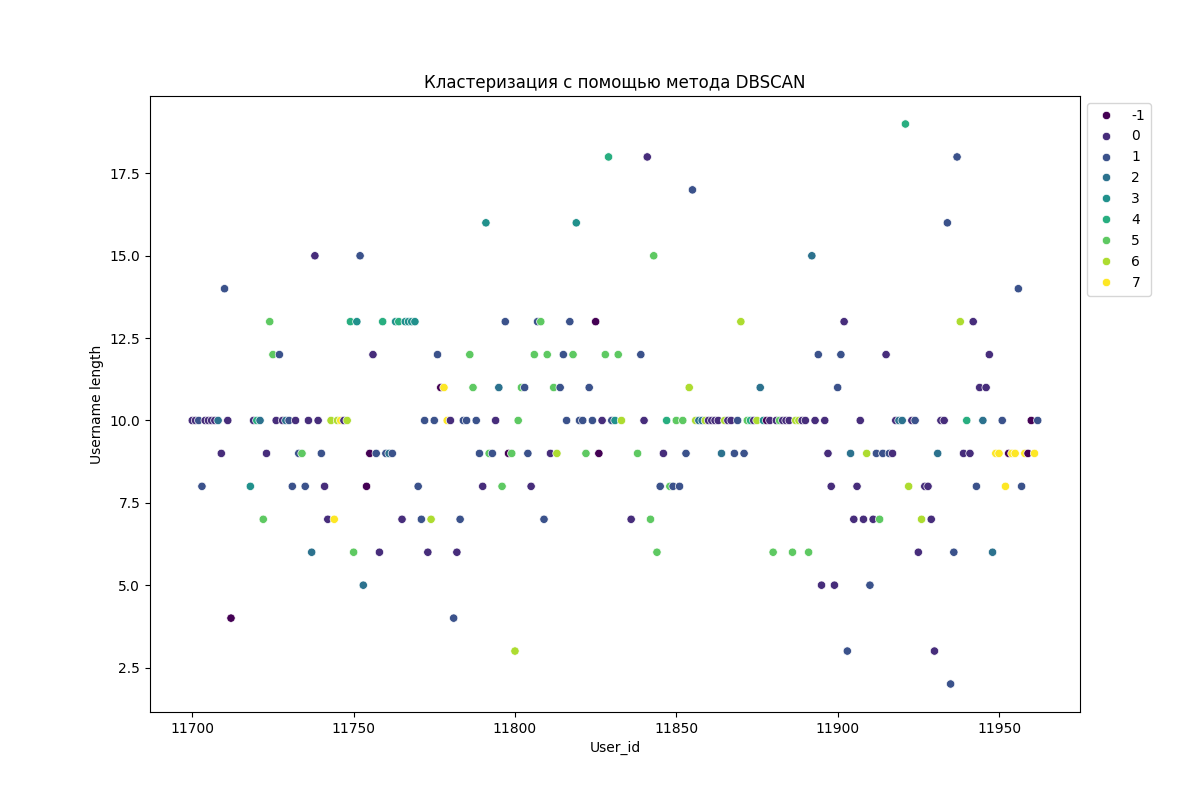
\includegraphics[scale=0.5]{Курсовая работа/pic/dbscan_clustering_ALL.png}
    \caption{Иерархическая кластеризация}
    \label{ris:dbscan}
\end{figure}

После этого были произведены расчеты метрик алгоритма, с использованием ячеек матрицы ошибок (табл. ~\ref{tabular:tableDBSCAN1}). 

\begin{table}[!ht]
    \onehalfspacing \caption{Матрица ошибок}
    \medskip
    \begin{tabular}{c|cc}
        & \text{Positive} & \text{Negative} \\
        \hline
        \text{True} & \text{7} & \text{155} \\
        \text{False} & \text{2} & \text{90} \\
    \end{tabular}
    \label{tabular:tableDBSCAN1}
\end{table}

$$
accuracy = \frac{TP+TN}{TP+TN+FP+FN} = 0,60
$$

$$
precision = \frac{TP}{TP+FP} =  0,3
$$

$$
recall = \frac{TP+TN}{TP+FN} = 0,03
$$

$$
F\text{-}measure = 2\cdot \frac{precision \cdot recall}{precision+recall} = 0,05
$$

\vspace{1.5em}
Расчеты метрик алгоритма, который работал со всеми признаками, включая признаки <<соседства>>. Матрица ошибок представлена в табл. ~\ref{tabular:tableDBSCAN2}

\begin{table}[!ht]
    \onehalfspacing \caption{Матрица ошибок}
    \medskip
    \begin{tabular}{c|cc}
        & \text{Positive} & \text{Negative} \\
        \hline
        \text{True} & \text{8} & \text{154} \\
        \text{False} & \text{3} & \text{89} \\
    \end{tabular}
    \label{tabular:tableDBSCAN2}
\end{table}

$$
accuracy = \frac{TP+TN}{TP+TN+FP+FN} = 0,64
$$

$$
precision = \frac{TP}{TP+FP} =  0,73
$$

$$
recall = \frac{TP+TN}{TP+FN} = 0,08
$$

$$
F\text{-}measure = 2\cdot \frac{precision \cdot recall}{precision+recall} = 0,14
$$

\vspace{1.5em}
\textbf{Сравнение результатов алгоритмов}

Результаты рассчитанных метрик для всех реализованных алгоритмов представлены в таблице ~\ref{tabular:tableСomparison}.

\begin{table}[H]
    \onehalfspacing \caption{Метрики алгоритмов}
    \medskip
        \begin{tabular}{c|c|c|c|c}
            & accuracy & precision & recall & F-measure \\ \hline
            \multicolumn{5}{c}{Без признаков <<соседства>>} \\ \hline
            Isolation forest & 0,63 & 0,62 & 0,08 & 0,14 \\  \hline 
            Hierarchical clustering & 0,60 & 0,30 & 0,03 & 0,05 \\  \hline 
            DBSCAN & 0,64 & 0,78 & 0,07 & 0,13\\ \hline 
            \multicolumn{5}{c}{С признаками <<соседства>>} \\ \hline
            Isolation forest & 0,62 & 0,54 & 0,07 & 0,12 \\  \hline 
            Hierarchical clustering & 0,60 & 0,33 & 0,04 & 0,07 \\  \hline 
            DBSCAN & 0,64 & 0,73 & 0,08 & 0,14\\ 
        \end{tabular}
    \label{tabular:tableСomparison}
\end{table}

По данным результатам можно сделать вывод, что без дополнительных признаков больше подходят для обрнаружения фиктивных аккаунтов Isolation forest и DBSCAN, с признаками же выигрывает DBSCAN.

\subsection{Функциональное тестирование}
Провести тестирование на соответствие приложения предъявленным требованиям. 

\vspace{1.5em}
\subsection{Вычислительные эксперименты}
В данном разделе представлены вычислительные эксперименты для набора данных.